\chapter{Experimental results}\label{chapter:Results}
All the tests were performed on a MSI GL63 8RD laptop, using the version 2004 of Windows 10 Home as Operating System. AcCAPPCHA results are described in the following sections, analysing two aspect: the security efficiency and the usability.

\section{Security analysis}
The main tests were performed by analysing the response of AcCAPPCHA when the user is a human and when it is a bot. All the techniques, described in \myref{Section}{AcCAPPCHA:user_activity}, are tested and the strength against the attacks mentioned in Invisible CAPPCHA (see \myref{Section}{inv:attacks}) are analysed again for the new CAPPCHA.  

\subsection{Human detection}\label{Results:human}
The responses of AcCAPPCHA for a human user were tested in all the three possible operating modes (see \myref{Section}{AcCAPPCHA:user_activity}): 
\begin{itemize}
\item{Time correspondence}
\item{Character correspondence}
\item{Both time and character correspondence}
\end{itemize}
The first method is the most efficient and AcCAPPCHA usually detects the human activity of a user at first or second trial using it. Sometimes the correspondence isn't found at first trial because of background noise. The last two approaches based on deep learning require the reduction of the number of labels for the classification of a key.\\
In this way I limit the possible characters that user could use. Hence the password can be composed of lower case alphabetic characters, accented vowels or numbers (see \myref{Figure}{Results:keyboard}). For this reason, I trained again the network using less labels and only the audio files related to these labels. However the user can also type the backslash key $\mathtt{\setminus b}$ but the corresponding character isn't analysed in the final verification.\\
AcCAPPCHA still considers the 10 most probable labels, predicted by the neural network, for each audio peak during the insertion of the password. The prediction apparently seems to work better after the simplification but this happens only because the correct key of an audio peak has higher probability to be predicted on a subset of all the keys of the keyboard.\\
At the contrary of D. Asonov, R. Agrawal's conclusions\cite{keyboard_acoustic}, I notice that, using the deep learning techniques, there are many false negatives given by the similar sound produced by several keys. The reasons of their presence could be:
\begin{itemize}
\item{different parts of my keyboard plate produce similar sounds}
\item{the built-in microphone of my laptop is more affected by the noise than an external microphone}
\item{the movements of the user's hands influence the noise during the password insertion}
%WORN OUT = usurato
\item{some keys are more worn out than other} 
\end{itemize}
AcCAPPCHA was executed three times for both the passwords \texttt{bye5} and \texttt{hello35} and for each type of used features. As explained in \myref{Section}{AcCAPPCHA:client}, a human user has at most 3 attempts to be correctly classified as human during an execution of AcCAPPCHA. For each execution of AcCAPPCHA, the \myref{Table}{Results:verification} reports the number of the step in which a human user is correctly detected as a human using both the character and the time correspondences. If the number of the step is replaced by the string NO, it means that AcCAPPCHA wasn't able to understand that the user was a human during the three trials. For each entry of the table where the number of the step is different from one, I also reported the number of characters correctly predicted in all the previous steps.\\
According to the results in the table, the worst deep learning method is the one that uses the spectrograms and a pre-trained deep learning model to extract the features of a press peak.
\begin{figure}[H]
     \centering
	 \includegraphics[width=0.7\textwidth]{Images/Results/keyboard_less}
     \caption{\footnotesize{Keys to be used in the password (highlighted in green).}}\label{Results:keyboard}
\end{figure}
\begin{table}[h]
\centering\footnotesize
\begin{tabular}{ccc}
\hline
{\textbf{Feature type}}&{\texttt{\textit{bye5}}}&{\texttt{\textit{hello35}}}\\
\hline
\multirow{3}{*}{FFT of touch peak} & {2 (3)} & {1}\\
& {2 (3)} & {1}\\
& {1} & {1}\\
\hline
\multirow{3}{*}{FFT of touch and hit peaks} & {2 (3)} & {2 (6)}\\
& {2 (3)} & {1}\\
& {3 (3)} & {3 (5, 6)}\\
\hline
\multirow{3}{*}{Spectrogram of touch and hit peaks} & {NO (3, 3, 3)} & {NO (5, 5, 6)}\\
& {NO (2,3,3)} & {NO (6,6,6)}\\
& {NO (3,2,3)} & {NO (5,4,5)}\\
\hline
\end{tabular}
\caption{\footnotesize{Step number when the human user is correctly identified as a human by AcCAPPCHA (3=maximum).}}
\label{Results:verification}
\end{table}

\subsection{Bot detection}
I've tested the bot activity analysing the response generated by AcCAPPCHA. I emulated it using several approaches and using the username \texttt{RaffaDNDM} and its password \textbf{hello35}:
\begin{itemize}
\item{\textbf{Python program with} \texttt{popen} \textbf{communication}\\
this approach opens a subprocess and a communication through pipes with stdin and stdout streams of AcCAPPCHA. Supposing that the hacker obtained the credentials in some way, the bot communicates the username and the password to running CAPPCHA with only the time correspondence selected. In practice the strength of AcCAPPCHA against this attack is very high because the insertion of the password is managed by AcCAPPCHA using consecutive calls to \texttt{getwch()} in the Windows Operating system. \\
This function belongs to \texttt{msvcrt} module and takes one character at the time. This module guarantees also that the console I/O routines are not compatible with stream I/O or low-level I/O library routines. In the Windows operating systems, the output from these functions is always directed to the console and cannot be redirected through any kind of pipes.\\
The program easily accepts the username, because AcCAPPCHA acquires it using the standard \texttt{input()} function, and then it waits for the insertion of the password. Hence the CAPPCHA waits forever the insertion of the first character of the password because \texttt{popen} can't access to the stream analysed by \texttt{getwch()}. I didn't iterate the insertion of the password for the maximum number of possible trials because even at the first insertion, AcCAPPCHA doesn't see any action performed by the bot.
\begin{lstlisting}[language=python, showstringspaces=false, tabsize=4, basicstyle=\footnotesize, caption={\footnotesize{Bot using popen.}},label={Results:popen_bot}]
from subprocess import Popen
import sys
import msvcrt
from time import sleep

def popen_bot(username, password):
    #Subprocess that redirects pipes
    process = Popen('python3 AcCAPPCHA.py -t -plot',
    				shell=True, 
    				stdin=subprocess.PIPE,
    				stdout=subprocess.PIPE,
    				stderr=subprocess.STDOUT)

    #Wait until username could be inserted
    sleep(4)
    #Write username and password
    credentials = username.encode() + b'\r\n' + \
    			  password.encode() + b'\r\n'
    output = process.communicate(credentials)[0]
    
    print(output.decode())
\end{lstlisting}
}
\item{\textbf{Python program with} \texttt{pynput} \textbf{module}\\
Using this module, the bot can access directly the console, bypassing the stream limits of \textbf{msvcrt} character acquisition. To emulate the user, the bot program should start the execution and immediately after the hacker must open the working terminal with AcCAPPCHA running. Then each character of the password is inserted by the bot on the selected terminal, by emulating the press and the release of the corresponding key of the keyboard.\\
This scenario isn't realistic because it requires the management of terminal windows by a human user. However it was useful to establish if the insertion of the password by a malware is correctly classified as a bot activity.
\begin{lstlisting}[language=python, showstringspaces=false, tabsize=4, basicstyle=\footnotesize, caption={\footnotesize{Bot using pynput module.}},label={Results:pynput_bot}]
from pynput.keyboard import Key, Controller
from time import sleep

def input_bot(username, password):
    #Object for control of keyboard events
    keyboard = Controller()

    def press_release(char):
        keyboard.press(char)
        keyboard.release(char)

    #Wait that username could be inserted
    sleep(4)

    #username insertion
    for x in username:
        press_release(x)
    
    press_release(Key.enter)

    #Trials for password insertion
    count = 0
    while(count<3):
        sleep(5)
        
        for x in password:
            press_release(x)

        press_release(Key.enter)
        count += 1
\end{lstlisting}
}
\item{\textbf{Remote control of the PC}\\
the last test was performed by using the program \texttt{Team Viewer} and accessing directly the terminal on which the remote user will run AcCAPPCHA. This type of attack isn't realistic but it has only a testing purpose like the previous mentioned attack with the Python bot.}
\end{itemize}
In the last two approaches the audio files recorded by AcCAPPCHA are very similar and highlights the two most probable situations:
\begin{itemize}
\descItem{The noise during the noise evaluation is very high}{If this happens, no audio peaks can be found (see \myref{Figure}{Results:silence_img}).}
\descItem{The noise during the noise evaluation is very low}{If this happens, some audio peaks can be found, even if the user was a bot, because there is some noise during the password insertion. However these audio peaks don't have a time correspondence with the time instants stored during the password insertion (see \myref{Figure}{Results:noise_img}). The only case, in which a bot could authenticate it self, is when there is a sequence of audio peaks caused by the noise and the time between them is the same of the stored ones.\\
However this event isn't very probable because it is hard that there would be an high noise only during the insertion of the password and not during the noise evaluation. If no noise evaluation was performed, the attacker could also analyse the background noise of the user and find a periodic sequence of peaks. Then the hacker could type the characters with the same time intervals discovered in the previous noise pattern. This highlights the strength and the importance of the noise evaluation performed before the insertion of the password.}
\end{itemize}
The bots activity was tested only using time correspondence of AcCAPPCHA because this is the best method for the analysis of the user's activity (see \myref{Section}{Results:human}). The tests were not performed using only character correspondence because many false positives can be found. The character correspondence were not applied after the time correspondence because the bots already fail the first verification based on time instants.
\begin{figure}[H]
     \centering
	 \begin{subfigure}[b]{0.48\textwidth}
         \centering
         \includegraphics[width=\linewidth]{Images/Results/Bot/silence}
         \caption{\footnotesize{Bot with \texttt{pynput} module.}}
     \end{subfigure}
	 \hfill     
     \begin{subfigure}[b]{0.48\textwidth}
         \centering
         \includegraphics[width=\linewidth]{Images/Results/TeamViewer/silence}
         \caption{\footnotesize{Team Viewer.}}
     \end{subfigure}
     \caption{\footnotesize{Plot of audio during the password insertion with high noise during noise evaluation.}}\label{Results:silence_img}
\end{figure}
\begin{figure}[H]
     \centering
	 \begin{subfigure}[b]{0.48\textwidth}
         \centering
         \includegraphics[width=\linewidth]{Images/Results/Bot/noise}
         \caption{\footnotesize{Bot with \texttt{pynput} module.}}
     \end{subfigure}
	 \hfill     
     \begin{subfigure}[b]{0.48\textwidth}
         \centering
         \includegraphics[width=\linewidth]{Images/Results/TeamViewer/noise}
         \caption{\footnotesize{Team Viewer.}}
     \end{subfigure}
     \caption{\footnotesize{Plot of audio during the password insertion with low noise during noise evaluation.}}\label{Results:noise_img}
\end{figure}
\subsection{Strength against known attacks}\label{Results:attacks}
Following the analysis performed for Invisible CAPPCHA\cite{Invisible_CAPPCHA}, I analyse the strength of AcCAPPCHA against the following attacks:
\begin{itemize}
\descItem{Replay attack}
{The message is still concatenated with a nonce and then they are signed to guarantee a client would use a nonce only once. The server still prevents this type of attacks by refusing the second message from a client with a nonce already used by him.}
\descItem{Reverse engineering attack}
{The code working on the client must be kept secure by the File System. Even if the attacker could reverse code on server, the signature of the message and the TLS communication guarantee that this attack cannot be performed.}
\descItem{Human-solver relay attack}
{AcCAPPCHA is strong against this attack because there aren't additional tasks to be performed as in classical CAPTCHAs. Hence no challenges can be sent to remote human solver.}
\descItem{Brute force and password replay attacks}
{A single call to AcCAPPCHA performs at most 3 attempts of password insertion. Hence this type of attack couldn't be performed because if invalid credentials were inserted by the user for 3 times, AcCAPPCHA immediately blocks the user.
}
\descItem{Denial Of Service (DOS)}
{If a bot was detected by AcCAPPCHA for 3 times during the execution, the program will block also the next trials on the client side. Hence the server won't be overloaded, because the client will refuse next attempts without communicating any message to the server.}
\end{itemize}
After the analysis of side-channel attacks, I decided also to modify the messages transmitted between the client and the server (see \myref{Section}{AcCAPPCHA:communication_CS}). All the messages, included the POST requests, are padded with space characters such that an hacker cannot understand which string was sent in every step of the communication. In fact if padding isn't applied, as explained in \myref{Section}{SideCH:vicinity}, the attacker could analyse the size of the packets to understand which data were exchanged by the parties.

\subsection{Other security considerations}
I analyse also other important aspects that guarantee the security of AcCAPPCHA. The first one is the choice of the HTTP POST method instead of HTTP GET method. I choose the first one because it's more secure to exchange sensible information than the second one. In fact, the HTTP GET method is associated to an URL that could be easily stored in the Browser History, even if in my application I didn't exploit the browser while the client sends the HTTP request.\\
Another important aspect to be considered is that the File Systems of the client and the server must guarantee that the file \texttt{block.txt}, used to manage the block period of a user, the encryption keys and the certificates must be kept secure. The File System has to guarantee the protection of the spectrogram images because the application generates them, during the insertion of the password, and it stores them in a folder. Then AcCAPPCHA accesses the images in the path, using the pre-trained network, and it extracts the features from them. Hence the File System must guarantee that the folder with spectrogram images couldn't be accessed by other applications. A path, for which the same type of protection must be ensured, is the one containing the model of the trained neural network, used for the classification of the key presses.\\
Another consideration is about the microphone permission that the Windows Operating System asks the user at only the first execution of AcCAPPCHA. The programs that have access to the microphone, as AcCAPPCHA, are listed in \textbf{Settings > Privacy > Permissions > Microphone} on Windows 10. The user could also analyse the list to find a bot that was installed by an attacker on the Operating System and it's trying to access the microphone (e.g. trying to elude AcCAPPCHA verification).\\
I suggest every user to enable the microphone icon in \textbf{Settings > Personalisation > Taskbar > Turn system icons on or off} even if an attacker could disable it. In this way, every time that an application accesses the microphone resource, the user could see the icon on the taskbar if the option was previously enabled on the settings. If an attacker has remote control of the pc on which client-side AcCAPPCHA runs, the user could understand on Windows 10 that he's under attack by looking at the icon because the microphone is used by AcCAPPCHA.\\

\section{Usability}
The verification with deep learning techniques would be more strong if the predictions would be more accurate. A problem of this methods is that the neural network must be trained using the audio files related to the keys of a specific keyboard. This method limits the usability of the neural network to the type of keyboard used to record the training set.\\
To use the character correspondence on several keyboard, each producer of keyboards should record audio files produced by the key presses and he should share them. In this way the neural network could be easily trained on several keyboards, generating a trained set of weights for each of them. Then AcCAPPCHA could be extended to download the set of weights, related to the keyboard of the user, at the first execution of the application. This action could also bring to a malicious use of the downloaded data (e.g. an attacker could use them to produce an advanced key-logger). Hence the access to these datasets should be limited to AcCAPPCHA application.\\
I used also other input devices to test the usability of the best method used to very the identity of the user (time correspondence). At first I tested AcCAPPCHA using an external wireless keyboard (Logitech K480) and positioning it in front of my laptop. AcCAPPCHA was tested also considering the interaction of the user with the touch keyboard of Windows 10 using:
\begin{itemize}
\item{\textbf{Mouse (}Zelotes T90\textbf{)}\\
the time correspondence exploits the sound of each mouse click needed to select a key on the keyboard.}
\descItem{Touchpad}{this device also guarantees to perform the time correspondence exploiting the sound of each click on the touchpad, used to select a key. The only condition, required by AcCAPPCHA to work correctly, is that the user clicks the physical left button at the bottom side of the touchpad.}
\end{itemize}
Using these three devices, the results of the time correspondence were equal to the ones obtained using the keyboard of the laptop. Hence the time correspondence is very efficient and it works well in several scenarios because it's not related to the input hardware but only to the microphone. At the contrary character correspondence is limited to the hardware characteristics of the input device. 